\section{Implementation}\label{sec:02_impl}
% What
This section describes the most important parts of the implementation of the application. It highlihtes the databse structure, and the behaviour of the Beans.


\subsection{Database}\label{sec:02_impl_db}


\subsubsection{Entities}\label{sec:02_impl_db_entities}
% What
\Fig{fig:02_impl_db_entities} visualizes the UML diagram of the entities, used for the database.
% Overall
Overall, the database is used to save the following information:
\begin{itemize}
\item Accommodations which represent either an apartment or a hotel
\item Occupancy, represents the availability of an accommodation entity for a specific day
\item Reservation which represent a single reservation made by a user
\end{itemize}

% Figure
\begin{figure}[h]
\centering
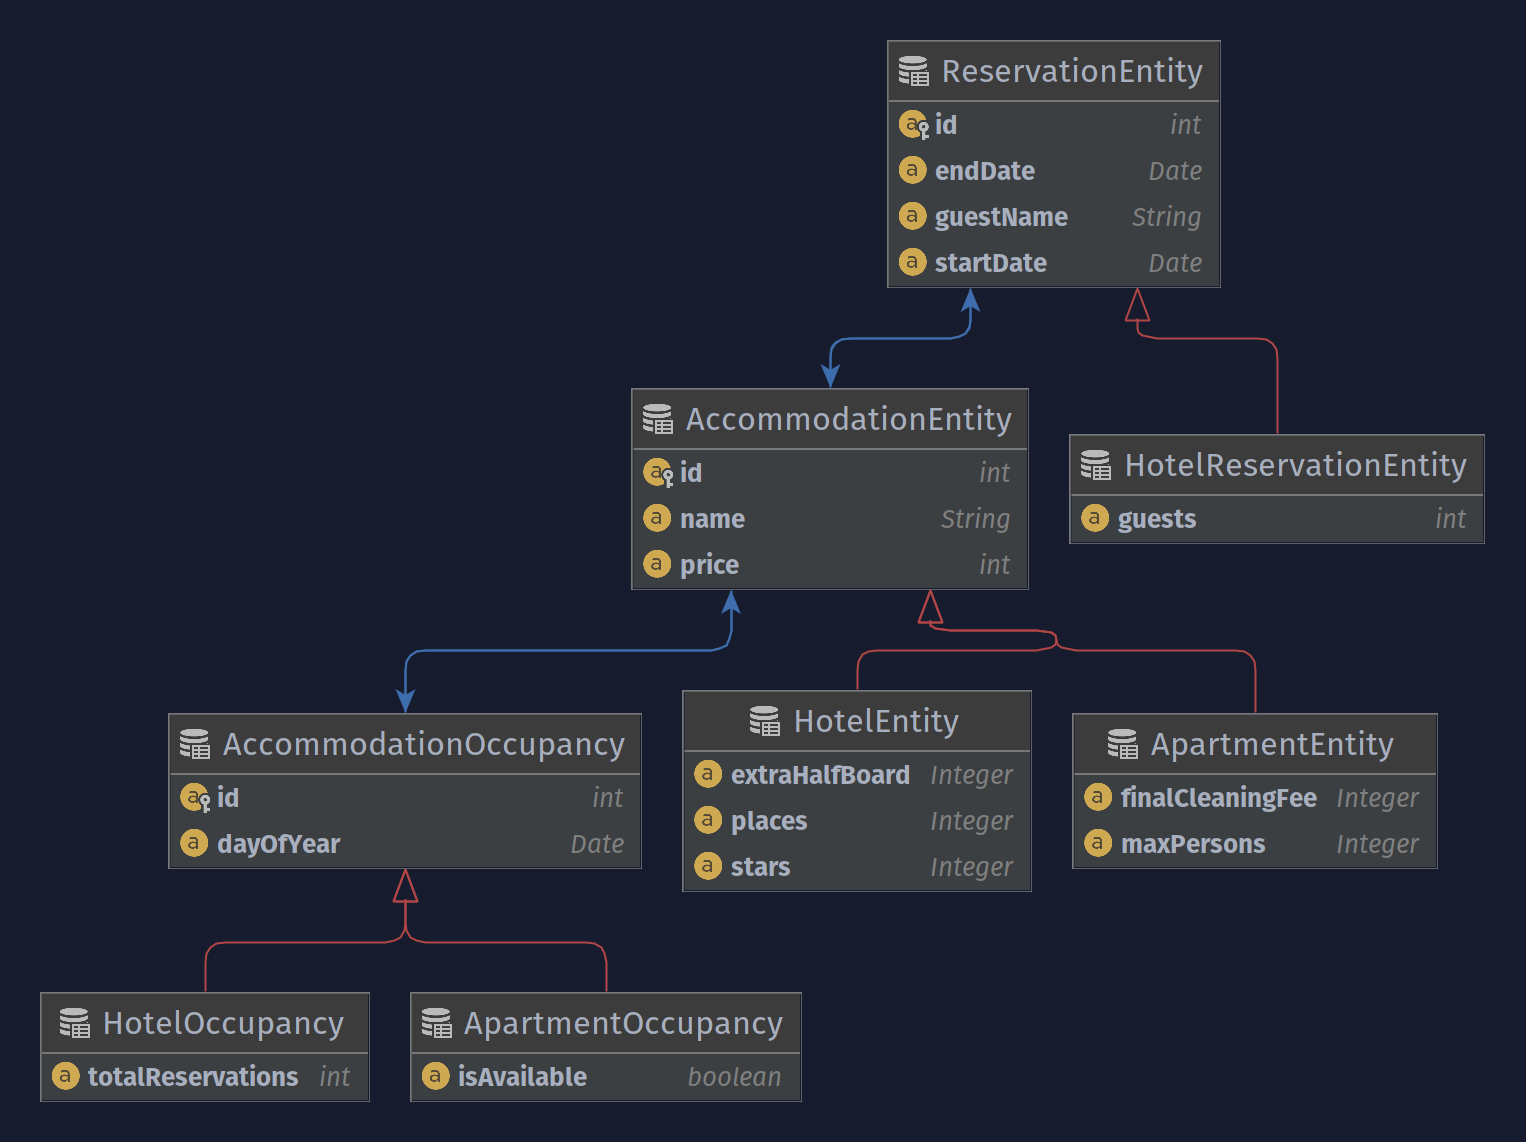
\includegraphics[scale=0.3]{images/02_impl/entities}
\caption{UML diagram of all database entities}
\label{fig:02_impl_db_entities}
\end{figure}

% Accommodatins
\paragraph{Accommodations}
Two types of accommodations exists for this application: Apartments and Hotels. 
% Properties
All accommadtions have a name, and a daily price. Additionally, an apartment has a final cleaning fee, an a number of maximum persons. A hotel has a rating of start, a number of free places, and a price for extra half-board.

% Classes
To implement the entities, an ApartmentEntity, and a HotelEntity have been implemented. Both classes inherit from the abstract AccommodationEntity class.


% Occupancies
\paragraph{Occupancies}
% What
Each accommodation needs an occupancy information for a specific date. The occupancy information describes if an accommodation is available on a specific date. The difference between an apartment and a hotel is, that a hotel has a specific number of reservation, and an aprtment is either available or unavaible, independetly of the number of persons.

% classes
To implement the occupancies, a parent class called HotelOccupancy exists, that includes only the date. Additionally, a class called ApartmentOccupancy saves the occupancies information for a hotel, which includes a boolean value called isAvailable that specifies, if the aprtment is avaiable for the specific date or not. Furthemore, a class called HotelEntity represent the occupancy of a hotel, which is a number of reservation for a specific date.


% Reservations
\paragraph{Reservations}
% What 
A user can make reservation that are saved to the database. A reservation consists of a start date and an end date that represent the date interval of the stay, and the name of the guest. These informations are saved by the ReservationEntity. Additionally, a classes called HotelReservationEntity, which inherits the ReservationEntity, is used to save the number of guests for on reservation of a hotel. An apartment does not need extra information, because it is either avaible or not, which is represented by the existance of a ReservationEntity in the table for the specific apartment for a specific date interval.


\subsubsection{Structure}\label{sec:02_impl_db_structure}
% What Tables
The database consists of three tables:
\begin{itemize}
\item Accommodation
\item Occupancy
\item Reservation
\end{itemize}
% For what
Each table is associated with an entity that are described in SEC XY.

% Explain Tables
\paragraph{Accommodation}
% Columns
FIG AB describes the structure of the Accommodation table. It is used to save the AccommodationEntity, as well as the child entities ApartmentEntity and HotelEntity.
% DB inheritance
To accomplish inheritance, the Single Table per Class Hierarchy strategy is used.

\paragraph{Occupancy}
% Figure
FIG BH describes the structure of the Occupancy table. It is used to save the OccupancyEntity and the HotelOccupancyEntity.
% Strategy
The Single Table per Class Hierarchy strategy is used as well to enable inheritance.

\paragraph{Reservation}
% Figure
FIG HJ describes the structure of the Reservations table. It saves the ApartmentEntity and the HotelEntity.
% Inheritance
For inheritance, it uses the Single Table per Class Hierarchy as well.


\subsubsection{Database Routine}\label{sec:02_impl_db_routine}
% Intro
A database routine needs to be implemented to seed the database, that is supposed to be used in the application.
% No EJB
This routine is not implemented as a EJB, instead, it will run as a standalone Java application.
% What data
The accommodations, as well as the occupancies of accommodatios are given by the task description.

% Technology
The following technologies are used to implement the database routine:
\begin{itemize}
\item Hibernate
\item JPA
\end{itemize}


% =====================
% =====================
\subsection{Enterprise Java Beans}\label{sec:02_impl_beans}
% Business logic
The business logic of this application is implemented using EJB 3. It is composed of three parts:
\begin{itemize}
\item \texttt{LocalDatabaseBean}
\item \texttt{AccommodationService}
\item \texttt{ReservationService}
\end{itemize}
% One Project
All services are part of a single Maven project called \textit{WebServices}.

% What
Each part (service) is an independent Baen. The client is able to lookup the Bean given an address and invoke methods on it. Only the Accommodation Service and the Reservation Service is available for the client. The Database Service is implemented using a local bean, because it is not intended, for the user, to interact with the database directly.


\subsubsection{LocalDatabaseBean}\label{sec:02_impl_beans_local}
% What
The \texttt{LocalDatabaseBean} is used to interact with the H2 database. It initiates the \texttt{EntityManager}, given by JPA, bu establishing a connection to a JTA datasource. Other services can use the Database Service to send queries and receive results from the database.

% How
As mentioned before, the Database Service is implemented as a \texttt{LocalBean}. Other Beans can interact with the Database Service using the Code-Injection pattern, which is shown in \Lst{lst:02_impl_ejb_db_cinjection}.
% The implementation
\begin{lstlisting}[label=lst:02_impl_ejb_db_cinjection, caption=Usage of the \texttt{LocalDatabaseBean} using Code-Injection, language=java]
@Stateless
@Remote(ReservationService.class)
public class ReservationBean implements ReservationService  {

    @EJB()
    private LocalDatabaseBean databaseBean;
    
    ...
    
}
\end{lstlisting}


\subsubsection{AccommodationService}\label{sec:02_impl_beans_acc}
% What
The Accommodation is used by the client to interact with the \texttt{AccommdationEntity} and its child classes \texttt{ApartmentEntity}, and \texttt{HotelEntity}. It uses the LocalDatabaseBean to send HQL queries to the H2 database.

% Getting available accommodations
Except from receiving accommodations based on specific properties, the most interesting part about the AccommodationService is how it receives available accommodations in a specific date range, given a number of guests.
% How
The idea is, that the number of occurencies of an accommadtion which is available in the specific date range, has to be qual the number of days of the given date range.
% SQL
\begin{lstlisting}[label=lst:02_impl_ejb_accommodation_sql, caption=Example of a HQL query to receive all available accommodations, language=sql]
SELECT a.accommodation
FROM AccommodationOccupancyEntity a
WHERE (
  ((a.isAvailable IS TRUE AND a.accommodation.maxPersons >= 2) 
  OR 
  ((a.accommodation.places - a.totalReservations) >= 2))
)
AND a.dayOfYear BETWEEN '2022-02-01' AND '2022-02-09'
GROUP BY a.accommodation.id
HAVING COUNT(*) = 9 
\end{lstlisting}
% Describe
\Lst{lst:02_impl_ejb_accommodation_sql} show an example HQL query implementation to get all available accommodations between 1. February 2022 and 10. February 2022 for 2 guests.
As described before, the \texttt{AccommodationOccupancyEntity} saves the occupancies of each accommodation for specific dates. Therefore, it is necessary to check for apartments if it is available, and has enough places for the number of guests. For hotels, it is necessary to check if the existing number of reservations minus the available places of that hotel is lower or equal the number of guests.
These constraints are checked for the range between the start date (1. February 2022) and the end date minus one day (9. February 2022). It is necessary to substract one day, because the guests will not stay for that day, and therefore the availability information for that day is unrelated.
After that it is important, thte the count of numbers of the accommodation, in that specific date range, is euqal to the number of days between the start and end date.


\subsubsection{ReservationService}\label{sec:02_impl_beans_reservation}
% Describe
To read from and write to the reservation table of the database, the ReservationService is used. It allows to persist new reservations to the database, and to get all reservations for a specific customer name.

% Adding new reservations
When adding a new reservation to the database, the \texttt{ReservationService} is also responsible to update the occupancies (mentioned in XY) of the selected accommodation. Then, it is necessary to add the number of guests, of the new reservation, to each entry of the accommodation occupancy.

% Calculating the price
Additionally, the ReservationService provides an interface to calculate the price of a reservation for either a Hotel or an Apartment.


\subsubsection{Build Process}\label{sec:02_impl_beans_build}
% Jar
The project is build using the \texttt{maven-ejb-plugin} maven plugin to create a EJB-Jar file.
% How
Then, the artifact can be built using the \texttt{mvn clean build} command.

% Settings
\Lst{lst:02_impl_ejb_buildprocess_pluginconfig} shows the configuration of the \texttt{maven-ejb-plugin} plugin.
% Config
\begin{lstlisting}[label=lst:02_impl_ejb_buildprocess_pluginconfig, caption=\texttt{maven-ejb-plugin} plugin configuration, language=xml]
<packaging>ejb</packaging>
...
<build>
  <finalName>${artifactId}.${version}</finalName>
  <plugins>
    <plugin>
      <groupId>org.apache.maven.plugins</groupId>
      <artifactId>maven-ejb-plugin</artifactId>
      <version>3.1.0</version>
    </plugin>
  </plugins>
</build>
\end{lstlisting}



% =====================
% =====================
\subsection{Web Application}\label{sec:02_impl_web}
% What parts

\subsubsection{Search}\label{sec:02_impl_web_search}

\subsubsection{Results}\label{sec:02_impl_web_results}

\subsubsection{Reservation Summary}\label{sec:02_impl_web_reservationsummary}

\subsubsection{Reservation Confirm}\label{sec:02_impl_web_reservationconfirm}

\subsubsection{My Reservations}\label{sec:02_impl_web_myreservations}
